%Input premable
\documentclass{beamer}

%Packages
\usepackage{graphicx}
\usepackage{graphics}
\usepackage{hyperref}
\usepackage[english]{babel}
\usepackage{amsmath}
\usepackage{amsfonts}
\usepackage{amssymb}
\usepackage{bm}
\usepackage{comment}
\usepackage{etoolbox}
\usepackage{graphicx}
\usepackage{tabularx,ragged2e,booktabs}
\usepackage{caption}
\usepackage{hyphenat}
\usepackage{fixltx2e}
\usepackage[para]{threeparttable}
\usepackage[capposition=top]{floatrow}
\usepackage{subcaption}
\usepackage{pdfpages}
\usepackage{natbib}
\usepackage{rotating}

%Math Functions
\DeclareMathOperator{\var}{Var}
\DeclareMathOperator{\cov}{Cov}

%Commands
\newcommand\independent{\protect\mathpalette{\protect\independenT}{\perp}}
\def\independenT#1#2{\mathrel{\rlap{$#1#2$}\mkern2mu{#1#2}}}
\newcommand{\overbar}[1]{\mkern 1.5mu\overline{\mkern-1.5mu#1\mkern-1.5mu}\mkern 1.5mu}
\newcommand{\equald}{\ensuremath{\overset{d}{=}}}

\newenvironment{wideitemize}{\itemize\addtolength{\itemsep}{10pt}}{\enditemize}

\mode<presentation>
	{
	\usetheme{UChicagoJorge}
	\setbeamercovered{transparent = 28}
	}

%\usecolortheme{UChicagoJorge} 
%\useinnertheme{UChicagoJorge}
%\useoutertheme{UChicagoJorge}

\title{Consumption \& Earnings Dynamics 1}
\subtitle{Econ 350, The University of Chicago}
\author{Jorge L. Garc\'{i}a}
\date{\today}



\begin{document}


\begin{frame}[plain]
	\titlepage
\end{frame}


\AtBeginSection[]
{
   \begin{frame}
       \frametitle{Outline}
       \tableofcontents[currentsection]
   \end{frame}
}

\section{Motivation}

\begin{frame}
	\frametitle{Main Questions}
\begin{itemize}
	\item How do the dynamics of earnings affect consumption choices over the life cycle?
		\begin{itemize}
			\item How much risk do households face?
			\item To what extent does risk affects basic household choices?
			\item What types of risk matter in explaining the behavior of households?		
		\end{itemize}
	\item Risk:
			\begin{itemize}
				\item What we commonly call uncertainty
				\item Agents are not aware of the realized states
				\item Agents have perfect information on the particular distribution that generates the states
			\end{itemize}
	\item Uncertainty:
			\begin{itemize}
				\item Agents ignore the states as well as the distribution that generates them
			\end{itemize}
\end{itemize}
\end{frame}

\begin{frame}
	\frametitle{Basic Concepts}
\begin{itemize}
	\item \textit{Ex-ante} and \textit{ex-post} responses to income variations
	\item \textit{Transitory} and \textit{permanent} income shocks
	\item \textit{Predictable} and \textit{unpredictable} income shocks
	\item Not only technicalities
		\begin{itemize}
			\item Differ conceptually
			\item Need different tools to tract them
		\end{itemize}
\end{itemize}
\end{frame}

\section{Benchmark Model}

\begin{frame}
	\frametitle{The PIH Model}
		\begin{itemize}
			\item Benchmark model in this literature: life-cycle permanent income hypothesis (PIH)
			\begin{itemize}
				\item Based on Friedman (1957)
				\item Quadratic preferences (what does this imply?)
				\item Consumers discount and interest rate satisfy $r(1 - \beta) = 1$
				\item Single risk free bond pays $r$
				\item Perfect capital markets
				\item Time horizon: $j = 1, \ldots, A$
				\item Information set and income of consumer $i$, at age $a$, in time $t$: $\Omega_{i,a,t}, Y_{i,a,t}$
				\item Summary equation of the model:
				\begin{equation}
				\Delta C_{i,a,t} = \pi_{a} \sum \limits _{j=0} ^{A} \frac{\mathbb{E}\left( Y_{i,a+j,t+j}| \Omega_{i,a,t}\right) - \mathbb{E}\left( Y_{i,a+j,t+j}| \Omega_{i,a-1,t-1}\right)}{(1+r)^j} \nonumber
				\end{equation}
			\end{itemize}
		\end{itemize}
\noindent where $\pi_{a}=\dfrac{r}{1+r} \left[ 1-\dfrac{1}{(1+r)^{A-a+1}} \right]^{-1}$
\end{frame}

\begin{frame}
	\frametitle{The PIH Model (contd 1)}
		\begin{itemize}
			\item Innovations to current and future income that arrive at $a$ potentially change consumption between $a$ and $a-1$
			\item Anticipated changes does not change anything: consumption smoothing!
			\item Key discussion: how to model the income process (lots of papers on this in the reading list)?
			\item Benchmark in Macro:
			\begin{eqnarray}
			Y_{i,a,t} &=& p_{i,a,t} + \varepsilon_{i,a,t} \nonumber \\
			p_{i,a,t} &=& p_{i,a-1,t-1} + \zeta_{i,a,t} \nonumber
			\end{eqnarray}
			\item Permanent shock: $\zeta_{i,a,t}$
			\item Transitory shock: $\varepsilon_{i,a,t}$
		\end{itemize}
\end{frame}

\begin{frame}
	\frametitle{The PIH Model (contd 2)}
		\begin{itemize}
			\item Under this specification
				\begin{equation}
					\Delta C_{i,a,t} = \pi_{a} \varepsilon_{i,a,t} + \zeta_{i,a,t} 
				\end{equation}
				\begin{itemize}
			\item Consumption responses:
					\begin{enumerate}
						\item One-to-one for permanent shocks
						\item Proportional-to-$\pi_{a}$ for transitory shocks
					\end{enumerate}
				\end{itemize}
		\end{itemize}
			
\begin{center}
\begin{figure}[H]
\caption*{The Response to Transitory Shocks in the PIH Model}
\centering
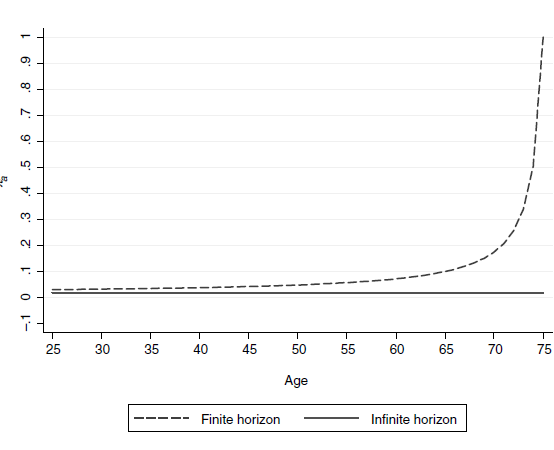
\includegraphics[width=1.2in, height=1.2in]{Figure1MP_2011.png}
\floatfoot{\begin{small}
\begin{tiny} Source: Meghir and Pistaferri (2011) \end{tiny}
\end{small}}
\end{figure}
\end{center}		
		
\end{frame}

\begin{frame}
	\frametitle{The PIH Model (contd 3)}
		\begin{itemize}
			\item Series of caveats:
			\begin{itemize}
				\item Consumers tend to follow the theory when expected income changes are large
					\begin{itemize}
						\item May be due to transaction costs
						\item Leads to ``smoothing excess''
					\end{itemize}
				\item Quadratic preferences
					\begin{itemize}
						\item Rule out precautionary savings
						\item Convenient for analytic terms
						\item Euler equations get very complicated with power utility functions (e.g, Blundell et al. (2012))		
					\end{itemize}
			\end{itemize}
		\end{itemize}
\end{frame}

\section{Learning about Risk}

\begin{frame}
		\frametitle{Two Approaches to Learn about Risk}
	\begin{enumerate}
		\item Identify insurance for a given information set:
			\begin{itemize}
				\item Assume a process for income, and therefore for consumption
				\item The assumptions imply an information set
				\item Estimate the parameters of the income and consumption processes
				\item Estimate insurance with respect to permanent and transitory shocks			
			\end{itemize}
		\item Identify and information set given and insurance configuration
			\begin{itemize}
				\item Basic concern
				\begin{itemize}
					\item Study superior information
					\item Agents may know more about shocks that the econometrician
					\item This may cause the econometrician to misinterpret consumption patterns and conclude smoothing excess
				\end{itemize}
					\item Various approaches to deal with this
						\begin{itemize}
					\item Browning et al. (1999): allow for econometrician ignorance in the income process
					\item Cunha et al (2005) and Cunha and Heckman (2007): distinguish wage variability and risk; model information
						\end{itemize}
			\end{itemize}
	\end{enumerate}
\end{frame}


\section{Consumption, Income, and Insurance}
\begin{frame}
	\frametitle{The Income Process}
	\begin{itemize}
		\item Simple framework to understand insurance against income shocks, based on BPP (2008)
		\item Permanent-transitory decomposition of residual log- income process
			\begin{eqnarray}
y_{i,t} &=&  P_{i,t} + t_{i,t} \nonumber \\
P_{i,t} &=& P_{i,t-1} + \xi_{i,t} \nonumber \\
t_{i,t} &=& \sum \limits _{j=0} ^q \theta_{j} \epsilon_{i,t-j} \nonumber
			\end{eqnarray}
			\item Leads to
			\begin{equation}
\Delta y_{i,t} = \xi_{i,t} + \Delta t_{i,t} \nonumber
			\end{equation}
	\end{itemize}
\end{frame}

\begin{frame}
	\frametitle{The Consumption Process and Insurance}
	\begin{itemize}
		\item Write residual log-consumptions as
		\begin{equation}
\Delta c_{i,t} = \phi_{i,t} \xi_{i,t} + \varphi_{i,t} \epsilon_{i,t} + \eta_{i,t} \nonumber \label{eq:conpro}
		\end{equation} 

		\item Insurance Alternatives:
			\begin{enumerate}
				\item Complete Markets Hypothesis ($\phi_{i,t} = \varphi_{i,t} = 0$): perfectly smooth out permanent and transitory shocks
				\item Autarky ($\phi_{i,t} = \varphi_{i,t} = 1$): change in consumption has a one-to-one response on both permanent and transitory shocks
				\item Incomplete Markets Hypothesis ($0 < \phi_{i,t} , \varphi_{i,t} < 1$): partial insurance against both income shocks
\end{enumerate}
	\end{itemize}
\end{frame}

\begin{frame}
	\frametitle{Identification}
	\begin{itemize}
		\item Three conditions suffice to identify the insurance coefficients and the variance of the income shocks
		\begin{enumerate}
			\item Transitory shocks to income are MA(0)
				\begin{equation}
					t_{i,t} = \epsilon_{i,t} \nonumber
				\end{equation}
			\item No Advance Information: 
				\begin{equation}
\cov(\Delta c_{i,t}, \xi_{i,t+1}) = \cov(\Delta c_{i,t}, \epsilon_{i,t+1}) = 0 \nonumber
				\end{equation}
			\item Short Memory: 
				\begin{equation}
\cov(\Delta c_{i,t}, \xi_{i,t-1}) = \cov(\Delta c_{i,t}, \epsilon_{i,t-2}) = 0 \nonumber
				\end{equation}
		\end{enumerate}
	\end{itemize}
\end{frame}

\begin{frame}
	\frametitle{Identification (contd)}
		\begin{itemize}
			\item Variance of transitory shocks
				\begin{equation}
					\var(\epsilon_{t}) = -\cov(\Delta y_{i,t}, \Delta y_{i,t+1}) \nonumber
				\end{equation}
			\item Variance of permanent shocks
				\begin{equation}
					\var(\xi_{t} ) = \cov(\Delta y_{i,t}, \Delta y_{i,t-1} + \Delta y_{i,t} + \Delta y_{i,t+1}) \nonumber
				\end{equation}
			\item Insurance coefficient against transitory shocks
				\begin{equation}
					\varphi_{i,t} = \frac{\cov(\Delta c_{i,t}, \Delta y_{i,t+1})}{\cov(\Delta y_{i,t}, \Delta y_{i,t+1})} \nonumber
				\end{equation}
			\item Insurance coefficient against permanent shocks
				\begin{equation}
					\phi_{i,t} = \frac{\cov(\Delta c_{i,t}, \Delta y_{i,t-1} + \Delta y_{i,t} + \Delta y_{i,t+1})}{\cov(\Delta y_{i,t}, \Delta y_{i,t-1} + \Delta y_{i,t} + \Delta y_{i,t+1})} \nonumber
				\end{equation}
		\end{itemize}
\end{frame}

\begin{frame}
	\frametitle{Evidence}
		\begin{itemize}
			\item BPP (2008) use PSID data from the late 1970s to the early 1990s to estimate the insurance coefficients 
		\end{itemize}

\begin{center}
\begin{figure}[H]
\caption*{Evidence on the Insurance Coefficients for the 1970s to the 1990s in the U.S.}
\centering
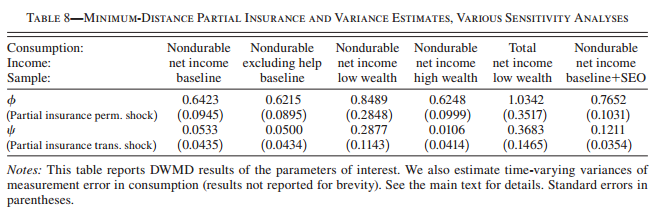
\includegraphics[width=3in, height=1in]{Table8BPP_2008.png}
\floatfoot{\begin{small}
\begin{tiny} Source: BPP (2008) \end{tiny}
\end{small}}
\end{figure}
\end{center}	

\end{frame}

\begin{frame}
	\frametitle{Next Steps}
		\begin{itemize}
			\item Study two papers that explore theoretical and empirical variations on this paper
				\begin{enumerate}
					\item Heathcote, Storesletten, and Violante (2013)
					\item Blundell, Pistaferri, and Saporta-Eksten (2013)
				\end{enumerate}
			\item See presentation Consumption \& Earnings Dynamics 2
		\end{itemize}

\end{frame}




\end{document}